\documentclass[a4paper,12pt]{article}
%%%%%%%%%%%%%%%%%%%%%%%%%%%%%%%%%%%%%%%%%%%%%%%%%%%%%%%%%%%%%%%%%%%%%%%%%%%%%%%%%%%%%%%%%%%%%%%%%%%%%%%%%%%%%%%%%%%%%%%%%%%%%%%%%%%%%%%%%%%%%%%%%%%%%%%%%%%%%%%%%%%%%%%%%%%%%%%%%%%%%%%%%%%%%%%%%%%%%%%%%%%%%%%%%%%%%%%%%%%%%%%%%%%%%%%%%%%%%%%%%%%%%%%%%%%%
\usepackage{eurosym}
\usepackage{vmargin}
\usepackage{amsmath}
\usepackage{graphics}
\usepackage{epsfig}
\usepackage{subfigure}
\usepackage{fancyhdr}
\usepackage{listings}
\usepackage{framed}
\usepackage{graphicx}
\usepackage{amsmath}
\usepackage{chngpage}
%\usepackage{bigints}

%\setcounter{MaxMatrixCols}{10}

\begin{document}
	\large
	%%-

%=========================================================================================================== %
\section*{Glyphs}
\begin{framed}
\noindent In the context of data visualization, a glyph is any marker, such as an arrow or similar marking, used to specify part of a scientific visualization. This is a representation to visualize data where the data set is presented as a collection of visual objects. These visual objects are collectively called a Glyph.
\end{framed}
Glyphs are the basic visual building blocks of Bokeh plots, e.g. lines, rectangles, squares, wedges, patches, etc. The \texttt{bokeh.plotting} interface provides a convenient way to create plots centered around glyphs.

\bigskip
\begin{itemize}
\item To style the fill, line, or text properties of a glyph, it is first necessary to obtain a specific \texttt{GlyphRenderer}. 

\item 
When using the \texttt{bokeh.plotting} interface, the glyph functions return the renderer:
\end{itemize}


\begin{framed}
\begin{verbatim}
>>> r = p.circle([1,2,3,4,5], [2,5,8,2,7])
>>> r
<bokeh.models.renderers.GlyphRenderer at 0x106a4c810>
\end{verbatim}
\end{framed}



%=========================================================================================================== %
Then, the glyph itself is obtained from the \texttt{.glyph} attribute of a \texttt{GlyphRenderer}:

\begin{framed}
	\begin{verbatim}
>>> r.glyph
<bokeh.models.markers.Circle at 0x10799ba10>
\end{verbatim}
\end{framed}
\newpage
% This is the object to set fill, line, or text property values for:

\begin{framed}
\begin{verbatim}
from bokeh.plotting import figure, output_file, show

output_file("axes.html")

p = figure(plot_width=400, plot_height=400)
r = p.circle([1,2,3,4,5], [2,5,8,2,7])
show(p)
\end{verbatim}
\end{framed}
\begin{figure}[h!]
\centering
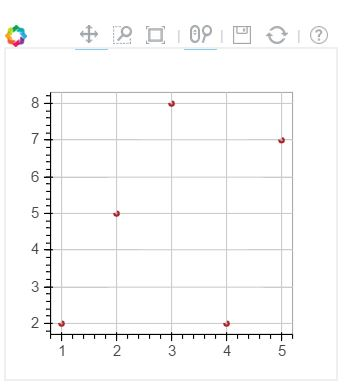
\includegraphics[width=0.7\linewidth]{images/04-glyphs-01}
\end{figure}
\newpage
\begin{framed}
	\begin{verbatim}
glyph = r.glyph
glyph.size = 60
glyph.fill_alpha = 0.2
glyph.line_color = "firebrick"
glyph.line_dash = [6, 3]
glyph.line_width = 2

show(p)
\end{verbatim}
\end{framed}
\begin{figure}[h!]
	\centering
	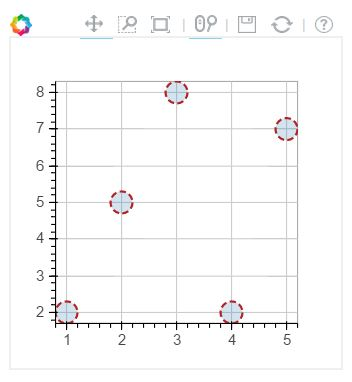
\includegraphics[width=0.7\linewidth]{images/04-glyphs-02}
\end{figure}
%=========================================================================================================== %
\newpage

\subsection*{Selected \& Unselected Glyphs}
The styling of selected and non-selected glyphs can be customized by setting the \texttt{selection\_glyph} and/or \texttt{nonselection\_glyph} attributes of the \texttt{GlyphRenderer} either manually or by passing them to \texttt{add\_glyph()}.

\begin{framed}
	\begin{verbatim}
from bokeh.io import output_file, show
from bokeh.plotting import figure
from bokeh.models import Circle

output_file("styling_selections.html")

p = figure(plot_width=400, plot_height=400, 
        tools="tap", title="Select a circle")
        
p.circle([1, 2, 3, 4, 5], [2, 5, 8, 2, 7], 
        size=50, name="mycircle")

selected_circle = Circle(fill_alpha=1, 
        fill_color="firebrick", 
        line_color=None)
        
nonselected_circle = Circle(fill_alpha=0.2, 
        fill_color="blue", 
        line_color="firebrick")

renderer = p.select(name="mycircle")
renderer.selection_glyph = selected_circle
renderer.nonselection_glyph = nonselected_circle

show(p)

\end{verbatim}
\end{framed}

%=========================================================================================================== %	
\begin{itemize}

\item Click/Tap to select circles on the plot above to see the effect on the nonselected glyphs.

\item Click in the plot, but not on a circle, to see their original state (this is set by the original call \texttt{p.circle()}).
\end{itemize}

The same could be achieved with the models interface as follows:


%=========================================================================================================== %
\begin{framed}
	\begin{verbatim}p = Plot()
source = ColumnDataSource(dict(x=[1, 2, 3], y=[1, 2, 3]))

initial_circle = Circle(x='x', y='y', 
			fill_color='blue', size=50)
			
selected_circle = Circle(fill_alpha=1, 
			fill_color="firebrick", line_color=None)
			
nonselected_circle = Circle(fill_alpha=0.2, 
			fill_color="blue", line_color="firebrick")

p.add_glyph(
  source,
  initial_circle,
  selection_glyph=selected_circle,
  nonselection_glyph=nonselected_circle
 )
\end{verbatim}
\end{framed}
%=========================================================================================================== %
\subsection*{Notes}
\begin{itemize}
\item Only the visual properties of \texttt{selection\_glyph} and \texttt{nonselection\_glyph} are considered when rendering. 
\item Changing positions, sizes, etc. will have no effect.
\end{itemize}


%=========================================================================================================== %

\end{document}